\documentclass{beamer}

\usepackage{amsmath}
\usepackage{amssymb}
\usepackage{amsthm}
\usepackage{tikz}
\usepackage{pgfplots}
\usepackage{graphicx}
\graphicspath{ {./img/} }

\usetheme{default}

\title{Inverting Vickrey}

\begin{document}

\begin{frame}{\titlepage}
  
\end{frame}

\begin{frame}{Intro}
  \only<-2>{
    We are assuming, as in (cite something) the cost function to be
    \begin{equation}
      \label{eq:cost}
      C(t_d) = \alpha tt(t_d) + \beta[t^*-t_d-tt(t_d)]^+ + \gamma[t_d+tt(t_d)-t^*]^+ 
    \end{equation}
  }
    \only<1>{
      where
      \begin{itemize}
      \item \(t^*\) is the desired arrival time
      \item \(\alpha\) is the value of time spent travelling
      \item \(\beta\) is the value of time spent waiting there
      \item \(\gamma\) is the value of time arriving late
      \item \(tt(t_d)\) is the expected (exogenous) travel time if leaving at time \(t_d\).
      \item \([x]^+ = \max(0, x)\)
      \end{itemize}
    }
    \only<2>{
      Without loss of generality, we can assume \(\alpha = 1\).

      Moreover, by defining the arrival time
      \begin{equation*}
        t_a = t_d + tt(t_d)
      \end{equation*}
      equation \eqref{eq:cost} becomes thus
    }
    \uncover<2->{
      \begin{equation}
        \label{eq:cost_ta}
        C(t_a) = tt_a(t_a) + \beta[t^*-t_a]^+ + \gamma[t_a-t^*]^+
      \end{equation}
    }
    \uncover<3>{
      We now assume the parameters \(\beta\), \(\gamma\) and the desired arrival times \(t^*\) to be normally distributed:
      \begin{itemize}
      \item \(\beta \sim \mathcal{N}(\mu_\beta, \sigma)\)
      \item \(\gamma \sim \mathcal{N}(\mu_\gamma, \sigma)\)
      \item \(t^* \sim \mathcal{N}(\mu_t, \sigma_t)\)
      \end{itemize}
    }
\end{frame}

\begin{frame}
  
  \begin{columns}
    \column{.4\linewidth}
      Drawing samples from these distributions, using a typical travel time function \(tt(t_a)\), the optima will be (in general) distributed as in the image,
      where the red and green zones roughly correspond to, respectively, early and late arrivals.

      Note that the x axis is random white noise, to better display the data distribution.
      Here the travel time function is shown, to demonstrate when these early and late arrivals actually occur.
    \column{.6\linewidth}
    \centering
      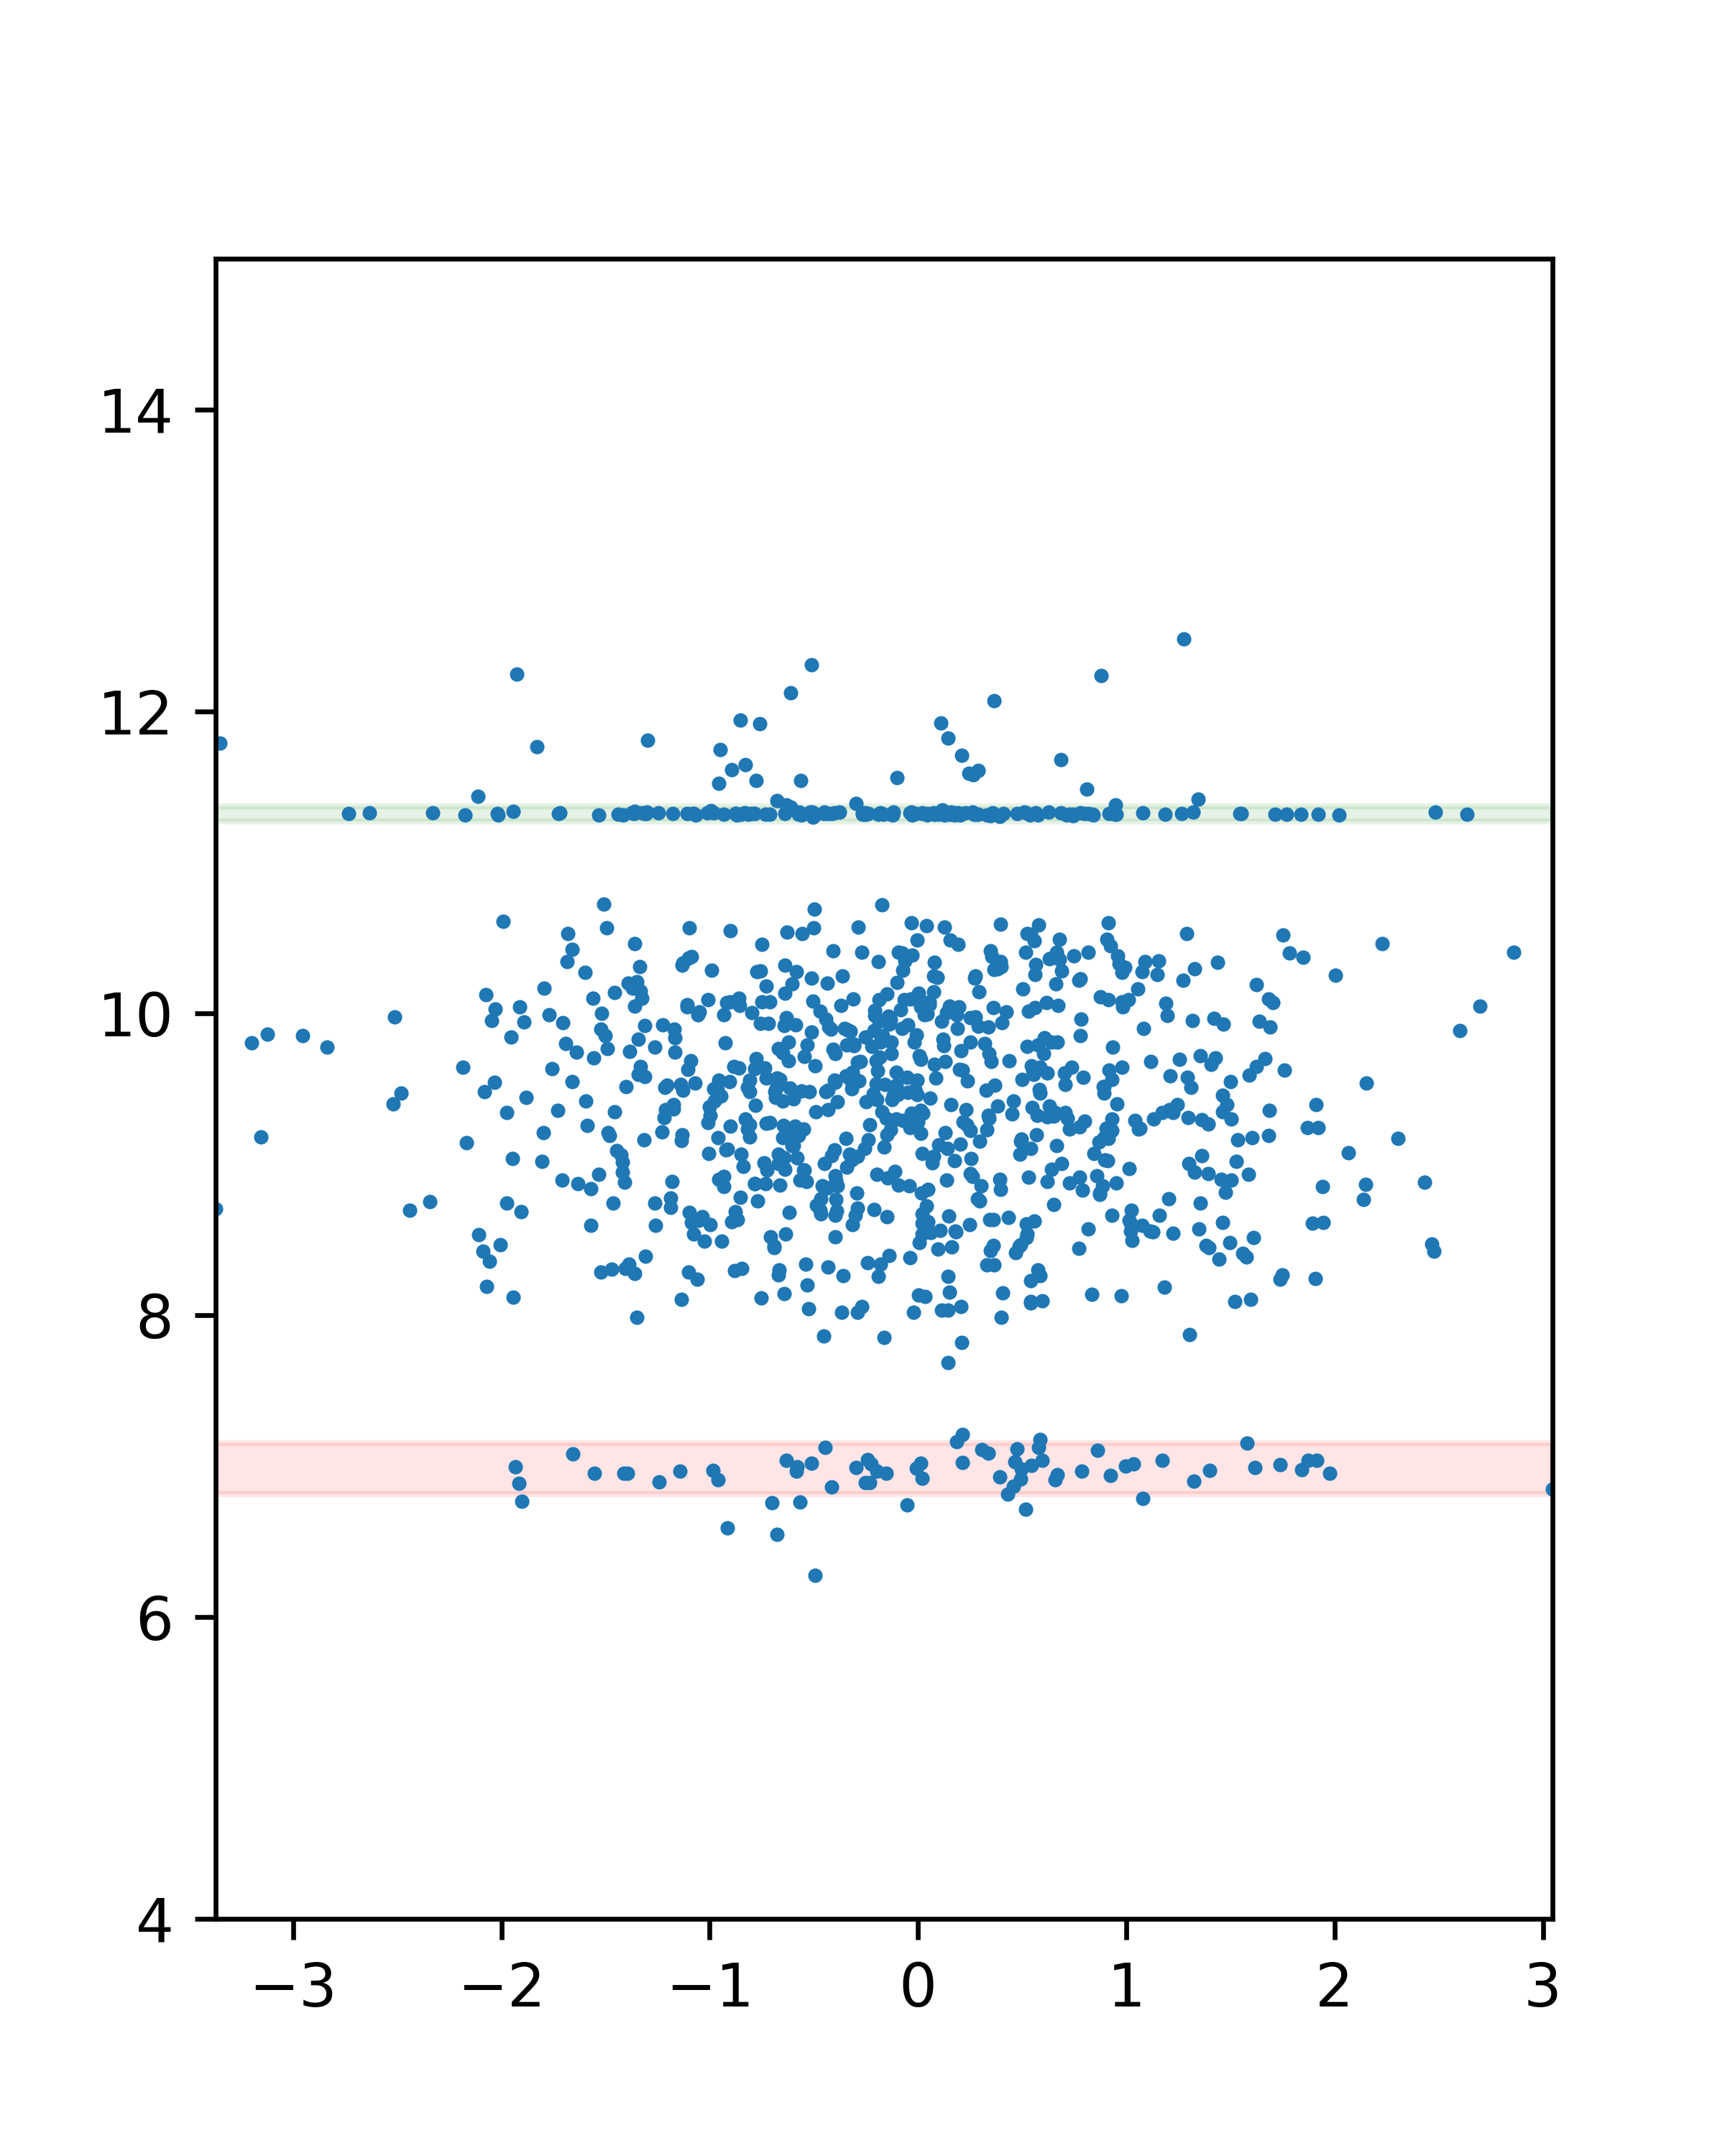
\includegraphics[width=\textwidth]{t_as}
  \end{columns}
\end{frame}

\begin{frame}
  As can be seen here, the early arrival are strictly correlated to the shape of the travel time function.
  \begin{center}
    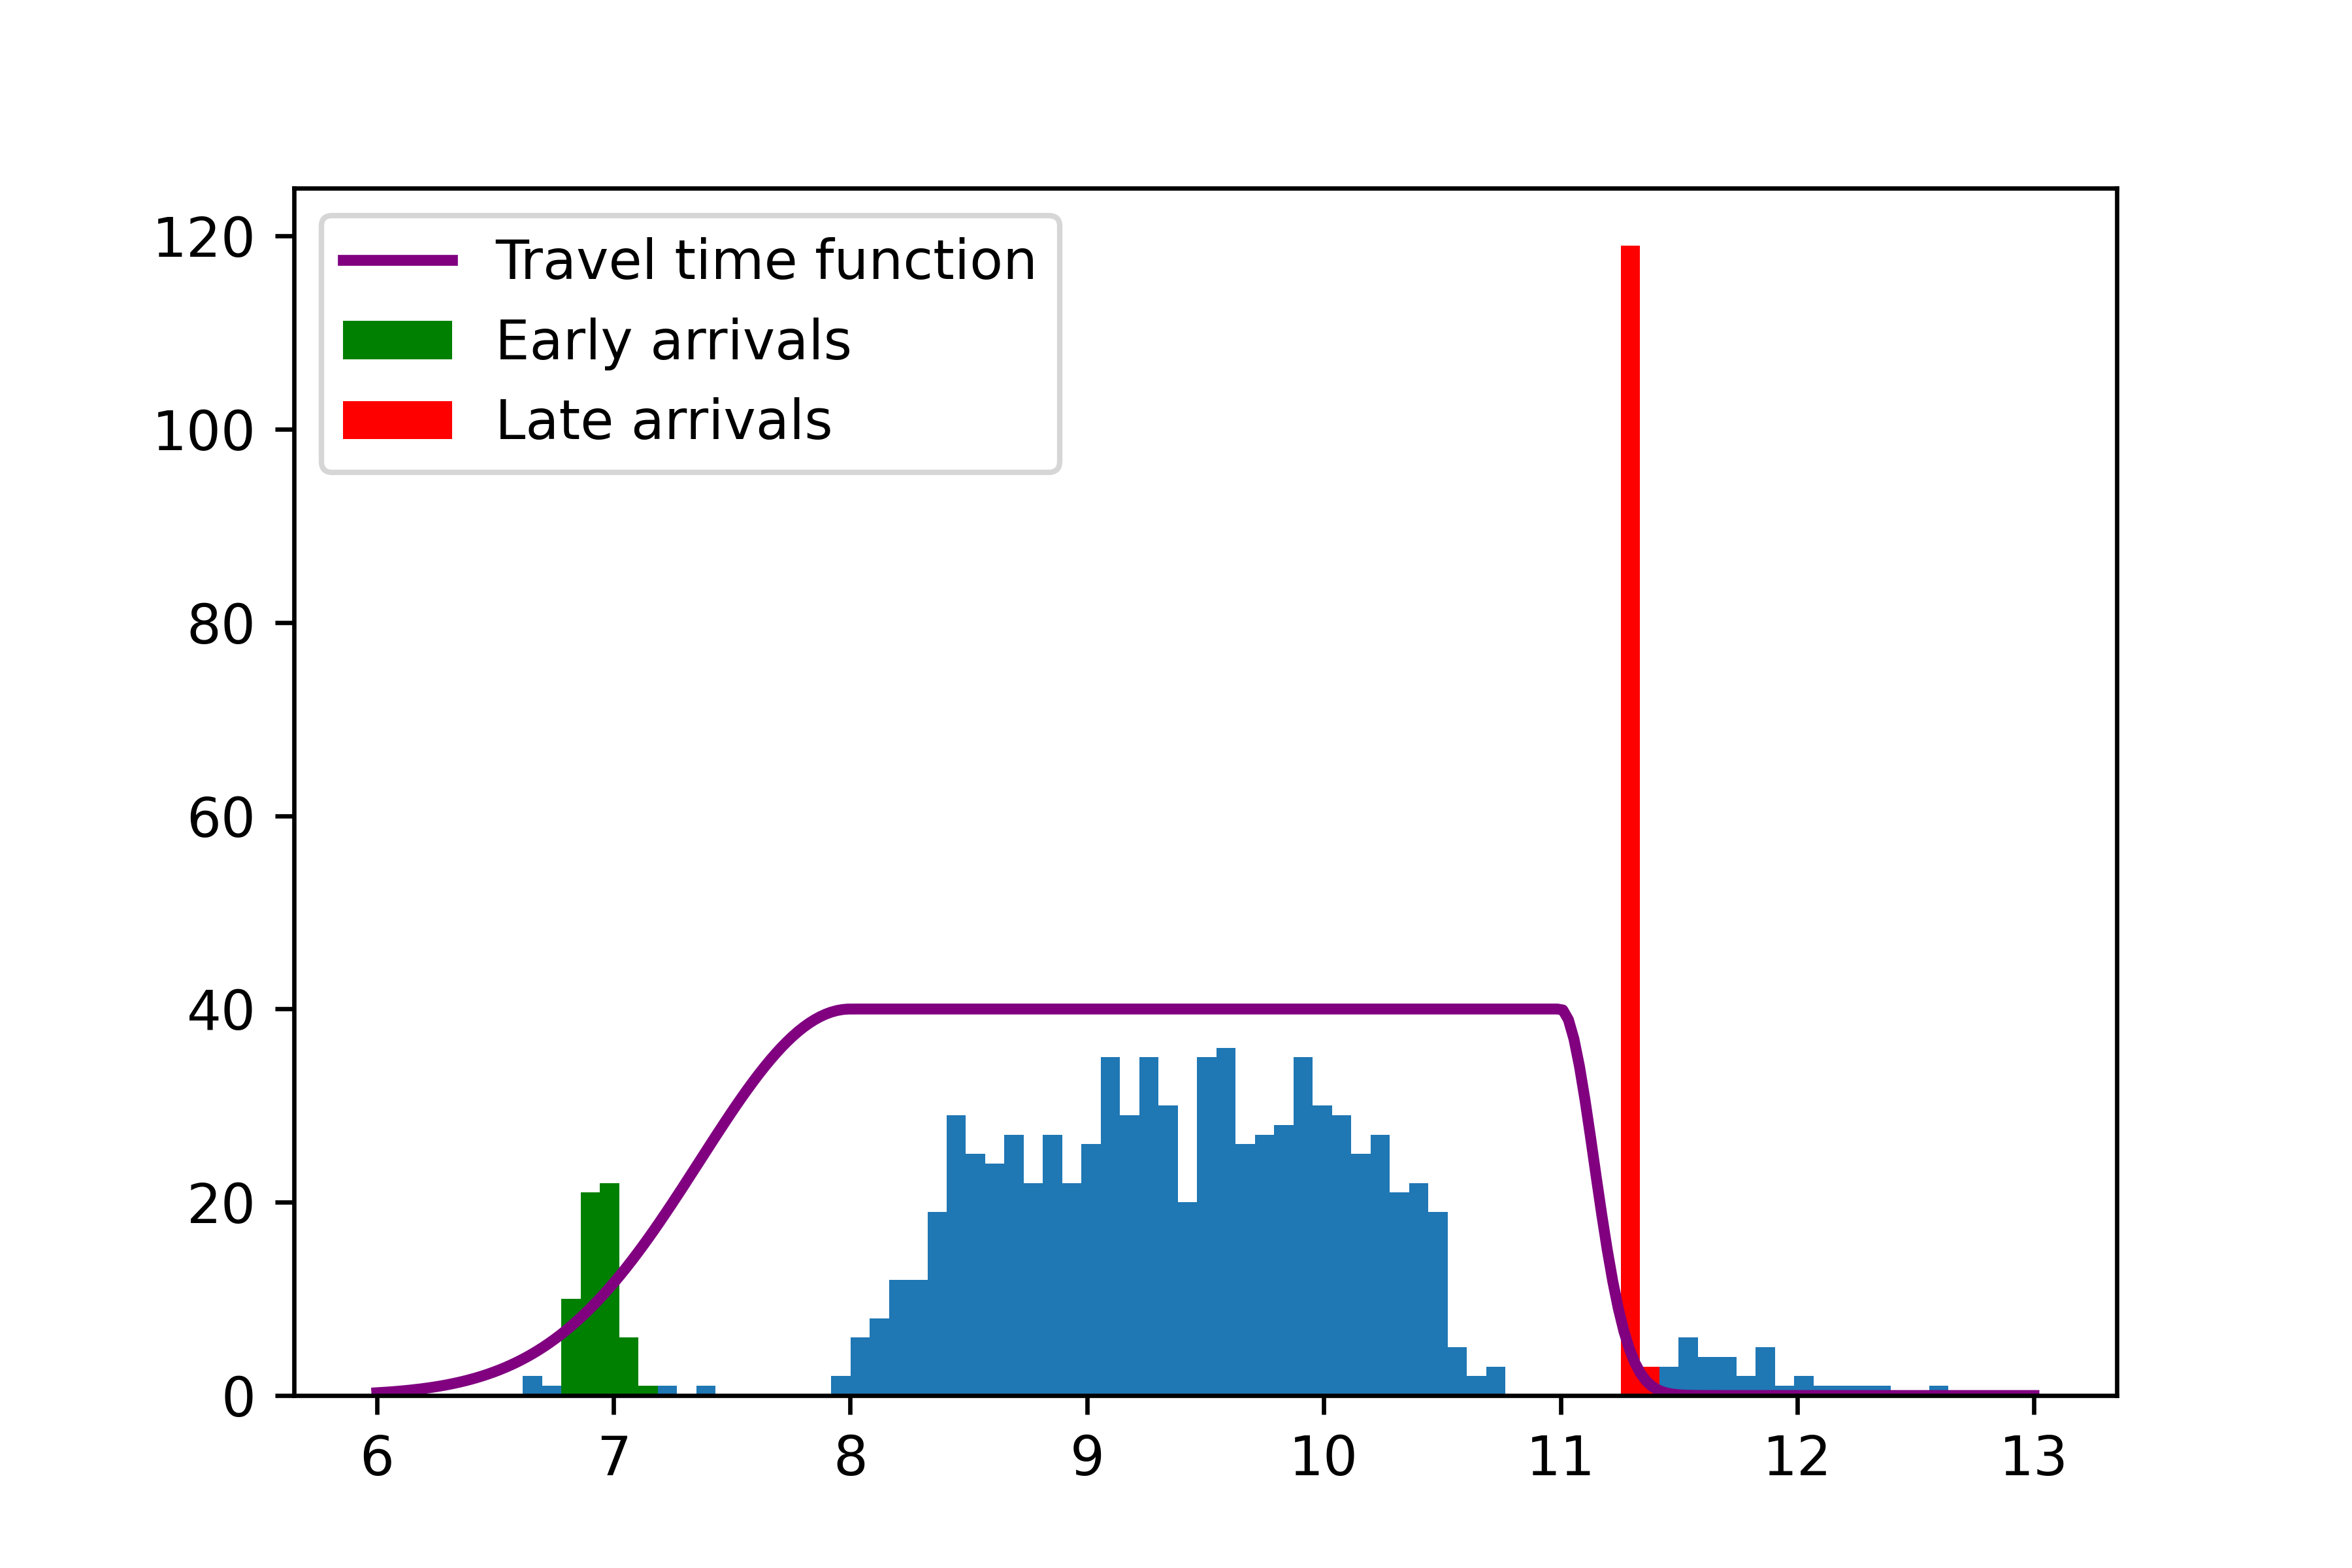
\includegraphics[width=\textwidth]{t_as_bins_tt}
  \end{center}
\end{frame}

\end{document}

%%% Local Variables:
%%% mode: LaTeX
%%% TeX-master: t
%%% End:
